\documentclass[fleqn, a4paper, 12pt, twoside]{article}
\usepackage{exsheets} %question and solution environments
\usepackage{amsmath, amssymb, amsthm} %standard AMS packages
\usepackage{esint} %integral signs
\usepackage{marginnote} %marginnotes
\usepackage{gensymb} %miscellaneous symbols
\usepackage{commath} %differential symbols
\usepackage{xcolor} %colours
\usepackage{cancel} %cancelling terms
\usepackage{siunitx} %formatting units
\usepackage{tikz, pgfplots} %diagrams
	\usetikzlibrary{calc, hobby, patterns, intersections, angles, quotes, spy}
\usepackage{graphicx} %inserting graphics
\usepackage{epstopdf} %converting and inserting eps graphics
\usepackage{hyperref} %hyperlinks
\usepackage{datetime} %date and time
\usepackage{ulem} %underline for \emph{}
\usepackage{xfrac, lmodern} %inline fractions
\usepackage{enumerate, enumitem} %numbered lists
\usepackage{float} %inserting floats
\usepackage[american voltages]{circuitikz} %circuit diagrams
\usepackage{pdflscape} %pages in landscape orientation
\usepackage{setspace} %double spacing
\usepackage{microtype} %micro-typography
\usepackage{listings} %formatting code
	\lstset{language=Matlab}
	\lstdefinestyle{standardMatlab}
	{
		belowcaptionskip=1\baselineskip,
		breaklines=true,
		frame=L,
		xleftmargin=\parindent,
		language=C,
		showstringspaces=false,
		basicstyle=\footnotesize\ttfamily,
		keywordstyle=\bfseries\color{green!40!black},
		commentstyle=\itshape\color{purple!40!black},
		identifierstyle=\color{blue},
		stringstyle=\color{orange},
	}
\usepackage{algpseudocode} %algorithms
\usepackage{algorithm} %algorithms
\usepackage{environ}
\usepackage{todonotes}

\renewcommand{\marginfont}{\scriptsize \color{red}}

\newcommand\numberthis{\addtocounter{equation}{1}\tag{\theequation}} %adds numbers to specific equations in non-numbered list of equations

\theoremstyle{definition}
\newtheorem{example}{Example}
\newtheorem{definition}{Definition}

\theoremstyle{theorem}
\newtheorem{theorem}{Theorem}
\newtheorem{law}{Law}

\newcommand{\curl}{\mathrm{curl\,}}

\newcommand{\divergence}{\mathrm{div\,}}

\makeatletter
\@addtoreset{section}{part} %resets section numbers in new part
\makeatother

\newcommand\blfootnote[1]{%
	\begingroup
	\renewcommand\thefootnote{}\footnote{#1}%
	\addtocounter{footnote}{-1}%
	\endgroup
}

\renewcommand{\tilde}{\widetilde}

\SetupExSheets{solution/print = true} %prints all solutions by default

% Uncomment to hide proofs
%\NewEnviron{killcontents}{}
%\let\proof\killcontents
%\let\endproof\endkillcontents

%opening
\title{Harmonic Analysis}
\author{Aakash Jog}
\date{2015-16}

\begin{document}

\maketitle
%\setlength{\mathindent}{0pt}

\blfootnote
{	
	\begin{figure}[H]
		\includegraphics[height = 12pt]{cc.eps}
		\includegraphics[height = 12pt]{by.eps}
		\includegraphics[height = 12pt]{nc.eps}
		\includegraphics[height = 12pt]{sa.eps}
	\end{figure}
	This work is licensed under the Creative Commons Attribution-NonCommercial-ShareAlike 4.0 International License. To view a copy of this license, visit \url{http://creativecommons.org/licenses/by-nc-sa/4.0/}.
} %CC-BY-NC-SA license

\tableofcontents

\newpage
\section{Lecturer Information}

\textbf{Barak Sober}\\
~\\
Office: Shenkar Physics 201\\
E-mail: \href{mailto:barakino@gmail.com}{barakino@gmail.com}\\
Telephone: \href{tel:+972 3-640-6024}{+972 3-640-6024}

\section{Required Reading}

\begin{enumerate}
	\item Folland, G.B.: Fourier Analysis and its applications, Wadsworth \& Brooks/Cole mathematics series, 1992
\end{enumerate}

\section{Additional Reading}

\begin{enumerate}
	\item Katznelson, Yitzhak. An introduction to Harmonic analysis. Cambridge University Press, 2004.
\end{enumerate}

\newpage
\part{Basic Definitions and Theorems}
\section{Sequences and Series}

\begin{definition}[Convergent series]
	The series $\sum\limits_{n = 0}^{\infty} a_n$ is said to converge if the sequence of partial sums $S_N = \sum\limits_{n = 0}^{N} a_n$ converges to a finite limit.
\end{definition}

\begin{definition}[Pointwise convergence of sequence of functions]
	Let $D \subseteq \mathbb{R}$, and $\{f_n(x) : D \to \mathbb{R}\}$ be a sequence of functions.
	$f_n(x)$ is said to converge pointwise, to a limit function $f(x)$ on $D$, if $\forall \varepsilon > 0$, $\forall x \in D$, $\exists N \in \mathbb{N}$, such that $\forall n > N$, $\left| f_n(x) - f(x) \right| < \varepsilon$.
\end{definition}

\begin{definition}[Uniform convergence of sequence of functions]
	Let $D \subseteq \mathbb{R}$, and $\{f_n(x) : D \to \mathbb{R}\}$ be a sequence of functions.
	$f_n(x)$ is said to converge uniformly to $f(x)$ on $D$ if $\forall \varepsilon > 0$, $\exists N \in \mathbb{N}$, such that, $\forall n > N$, $\forall x \in D$, $\left| f_n(x) - f(x) \right| < \varepsilon$.
\end{definition}

\begin{theorem}
	If $\left\{ f_n(x) \right\}_{n = 1}^{\infty}$ are continuous functions, and $f_n(x) \xrightarrow{U} f(x)$, then $f(x)$ is also continuous.
\end{theorem}

\begin{theorem}
	If a sequence of functions converges pointwise as well as uniformly, then the limit function must be the same.
\end{theorem}

\begin{theorem}[Weierstrass M-test]
	If $|u_k(x)| \le c_k$ on $D$ for $k \in \{ 1, 2, 3, \dots \}$ and the numerical series $\sum\limits_{k = 1}^{\infty} c_k$ converges, then the series of functions $\sum\limits_{k = 1}^{\infty} u_k(x)$ converges uniformly on $D$.
	\label{Weierstrass_M-test}
\end{theorem}

\section{Periodic Functions}

\begin{definition}[Periodic functions]
	A function $f : \mathbb{R} \to \mathbb{R}$ is said to be periodic if $\exists 0 < L \in \mathbb{R}$, such that $\forall x \in \mathbb{R}$,
	\begin{align*}
		f(x) & = f(x + L)
	\end{align*}
	If there exists a minimum $L$, it is called $L^*$, the fundamental period.
	\marginnote
	{
		For a function $f(x) = k$, as any positive number is a period, there is no minimum $L$.
		Hence, $\nexists L^*$.
	}
\end{definition}

\section{Odd and Even Functions}


\begin{definition}[Odd functions]
	A function is said to be odd if $f(-x) = -f(x)$.
	\marginnote
	{
		Odd functions are symmeteric about the origin.
	}
\end{definition}

\begin{definition}[Even functions]
	A function is said to be even if $f(-x) = f(x)$.
	\marginnote
	{
		Odd functions are symmeteric about the $y$-axis.
	}
\end{definition}

\begin{theorem}
	If $h(x)$ is odd,
	\begin{align*}
		\int\limits_{-L}^{L} h(x) \dif x & = 0
	\end{align*}
\end{theorem}

\newpage
\part{Introduction to Fourier Series}

\section{Real Fourier Series}

\begin{definition}
	Let $f : [-L,L] \to \mathbb{R}$, where $L > 0$.
	If $\forall x \in [-L,L]$, then
	\begin{align*}
		f(x) & = \frac{1}{2} a_0 + \sum\limits_{n = 1}^{\infty} \left( a_n \cos\left( \frac{n \pi}{L} x \right) + b_n \sin\left( \frac{n \pi}{L} x \right) \right)
	\end{align*}
\end{definition}

\begin{theorem}
	Let $L > 0$, $m \in \mathbb{W}$, $n \in \mathbb{W}$.\\
	Then
	\begin{align*}
		\int\limits_{-L}^{L} \cos\left( \frac{m \pi}{L} x \right) \cos\left( \frac{n \pi}{L} x \right) \dif x &=
			\begin{cases}
				0   & ;\quad m \neq n     \\
				L   & ;\quad m = n \neq 0 \\
				2 L & ;\quad m = n = 0    \\
			\end{cases}
	\end{align*}
\end{theorem}

\begin{proof}
	\begin{align*}
		E & = \int\limits_{-L}^{L} \cos\left( \frac{m \pi}{L} x \right) \cos\left( \frac{n \pi}{L} x \right) \dif x \\
                  & = \int\limits_{-L}^{L} \frac{1}{2} \left( \cos\left( (m + n) \frac{\pi}{L} x \right) + \cos\left( (m - n) \frac{\pi}{L} x \right) \right) \dif x
		\marginnote
		{
			$\because \cos \alpha \cos \beta = \frac{\cos(\alpha + \beta)}{2} + \frac{\cos(\alpha - \beta)}{2}$
		}
	\end{align*}
	If $m \neq n$,
	\begin{align*}
		E & = \frac{1}{2} \left. \left( \frac{\sin\left( (m + n) \frac{\pi}{L} x \right)}{(m + n) \frac{\pi}{L}} + \frac{\sin\left( (m - n) \frac{\pi}{L} x \right)}{(m - n) \frac{\pi}{L}} \right) \right|_{-L}^{L} \\
                  & = 0
	\end{align*}
	~\\
	If $m = n \neq 0$,
	\begin{align*}
		E & = \int\limits_{-L}^{L} \frac{1}{2} \left( \cos\left( 2 m \frac{\pi}{L} x \right) + 1 \right) \dif x                      \\
                  & = \frac{1}{2} \int\limits_{-L}^{L} \cos\left( 2 m \frac{\pi}{L} x \right) \dif x + \left. \frac{1}{2} x \right|_{-L}^{L} \\
                  & = L
	\end{align*}
	~\\
	If $m = n = 0$,
	\begin{align*}
		E & = \int\limits_{-L}^{L} \cos(0) \cos(0) \dif x \\
                  & = \left. x \right|_{-L}^{L}                   \\
                  & = 2 L
	\end{align*}
\end{proof}

\begin{theorem}
	Let $L > 0$, $m \in \mathbb{N}$, $n \in \mathbb{N}$.\\
	Then
	\begin{align*}
		\int\limits_{-L}^{L} \sin\left( \frac{m \pi}{L} x \right) \sin\left( \frac{n \pi}{L} x \right) \dif x &=
			\begin{cases}
				0 & ;\quad m \neq n \\
				L & ;\quad m = n    \\
			\end{cases}
	\end{align*}
\end{theorem}

\begin{theorem}
	Let $L > 0$, $m \in \mathbb{W}$, $n \in \mathbb{W}$.\\
	Then
	\begin{align*}
		\int\limits_{-L}^{L} \sin\left( \frac{m \pi}{L} x \right) \cos\left( \frac{n \pi}{L} x \right) \dif x & = 0
	\end{align*}
\end{theorem}

Assuming $f(x)$ is known, and assuming that it can be integrated term by term,
\begin{align*}
	\int\limits_{-L}^{L} f(x) \dif x            & = \int\limits_{-L}^{L} \frac{1}{2} a_0 \dif x + \sum_{n = 1}^{\infty} a_n \int\limits_{-L}^{L} \cos\left( n \frac{\pi}{L} x \right) \dif x + b_n \int\limits_{-L}^{L} \sin\left( n \frac{\pi}{L} x \right) \dif x \\
	\therefore \int\limits_{-L}^{L} f(x) \dif x & = \frac{1}{2} \int\limits_{-L}^{L} a_0 \dif x                                                                                                                                                                     \\
                                                    & = \frac{1}{2} a_0 \cdot 2 L                                                                                                                                                                                       \\
	\therefore a_0                              & = \frac{1}{L} \int\limits_{-L}^{L} f(x) \dif x
\end{align*}
Similarly, multiplying the series with $\cos\left( m \frac{\pi}{L} x \right)$ for $m \neq 0$ and integrating,
\begin{align*}
	a_m & = \frac{1}{L} \int\limits_{-L}^{L} f(x) \cos\left( m \frac{\pi}{L} x \right) \dif x
\end{align*}
for $m \in \mathbb{N}$.\\
Similarly, for $m \in \mathbb{N} \setminus \{0\}$,
\begin{align*}
	b_m & = \frac{1}{L} \int\limits_{-L}^{L} f(x) \sin\left( m \frac{\pi}{L} x \right) \dif x
\end{align*}

\begin{definition}
	The expansion
	\begin{align*}
		f(x) & \approx \frac{1}{2} a_0 + \sum\limits_{i = 1}^{\infty} \left( a_n \cos\left( n \frac{\pi}{L} x \right) + b_n \sin\left( n \frac{\pi}{L} x \right) \right)
	\end{align*}
	where, for $m \in \mathbb{N}$,
	\begin{align*}
		a_m & = \frac{1}{L} \int\limits_{-L}^{L} f(x) \cos\left( m \frac{\pi}{L} x \right) \dif x
	\end{align*}
	and, for $m \in \mathbb{N} \setminus \{0\}$,
	\begin{align*}
		b_m & = \frac{1}{L} \int\limits_{-L}^{L} f(x) \sin\left( m \frac{\pi}{L} x \right) \dif x
	\end{align*}
	is called the Fourier Series of $f(x)$.
\end{definition}

\section{Complex Fourier Series}

By Euler's formula,
\begin{align*}
	\cos \theta &= \frac{1}{2} \left( e^{i \theta} + e^{-i \theta} \right)\\
	\sin \theta &= \frac{1}{2 i} \left( e^{i \theta} - e^{-i \theta} \right)
\end{align*}
Therefore,
\begin{align*}
	\frac{1}{2 i} &= -\frac{i}{2}
\end{align*}
Therefore, substituting in the Fourier series,
\begin{align*}
	f(x) &\approx \frac{1}{2} a_0 + \sum\limits_{n = 1}^{\infty} \left( a_n \frac{1}{2} \left( e^{\frac{i n \pi}{L} x} + e^{-\frac{i n \pi}{L} x} \right) - b_n \frac{i}{2} \left( e^{\frac{i n \pi}{L} x} - e^{-\frac{i n \pi}{L} x} \right) \right)\\
	&\approx \frac{1}{2} a_0 + \sum\limits_{n = 1}^{\infty} \left( e^{\frac{i n \pi}{L} x} \left( \frac{1}{2} a_n - \frac{i}{2} b_n \right) + e^{-\frac{i n \pi}{L} x} \left( \frac{1}{2} a_n + \frac{i}{2} b_n \right) \right)\\
	&\approx \frac{1}{2} a_0 + \sum\limits_{n = 1}^{\infty} \left( e^{\frac{i n \pi}{L} x} \left( \frac{1}{2} a_n - \frac{i}{2} b_n \right) \right) + \sum\limits_{n = -\infty}^{1} \left( e^{\frac{i n \pi}{L} x} \left( \frac{1}{2} a_n + \frac{i}{2} b_n \right) \right)\\
	&\approx \sum\limits_{n = -\infty}^{\infty} c_n e^{\frac{i n \pi}{L} x}
\end{align*}

\section{Bessel's Inequality}

\begin{definition}[Piecewise continuous functions]
	$f : \mathbb{R} \to \mathbb{R}$ is said to be piecewise continuous if, for every finite interval $[a,b]$ there is a finite number of discontinuity points, and the one-sided limits at each of these points are also finite.
\end{definition}

\begin{definition}[Piecewise continuously differentiable functions]
	$f : \mathbb{R} \to \mathbb{R}$ is said to be piecewise continuously differentiable if it is piecewise continuous, and
	\begin{align*}
		\lim\limits_{h \to 0^+} \frac{f(x + h) - f(x^+)}{h} &< \infty
	\end{align*}
	and
	\begin{align*}
		\lim\limits_{h \to 0^-} \frac{f(x + h) - f(x^-)}{h} &< \infty
	\end{align*}
\end{definition}

\begin{theorem}[Bessel's Inequality]
	Let $f(x)$ be a piecewise continuous function defined on $[-L,L]$.
	Then
	\begin{align*}
		\frac{1}{2} {a_0}^2 + \sum\limits_{n = 1}^{\infty} {a_n}^2 + {b_n}^2 &\le \frac{1}{L} \int\limits_{-L}^{L} {f(x)}^2 \dif x
	\end{align*}
	\label{Bessel's_Inequality}
\end{theorem}

\section{Riemann-Lebesgue's Lemma}

\begin{theorem}[Riemann-Lebesgue's Lemma]
	If $f(x)$ is piecewise continuous on $[-L,L]$, then
	\begin{equation*}
		\lim\limits_{n \to \infty} a_n = \lim\limits_{n \to \infty} b_n = 0
	\end{equation*}
	\label{Riemann-Lebesgue's_Lemma}
\end{theorem}

\begin{proof}
	By \nameref{Bessel's_Inequality},
	\begin{align*}
		\frac{1}{2} {a_0}^2 + \sum\limits_{n = 1}^{\infty} {a_n}^2 + {b_n}^2 &\le \int\limits_{-L}^{L} {f(x)}^2 \dif x\\
		\therefore \frac{1}{2} {a_0}^2 + \sum\limits_{n = 1}^{\infty} {a_n}^2 + {b_n}^2 &< \infty
		\marginnote
		{
			As the function is piecewise continuous in $[-L,L]$, its integral from $-L$ to $L$ is finite.
		}
	\end{align*}
	Therefore,
	\begin{align*}
		\lim\limits_{n \to \infty} {a_n}^2 &\le \lim\limits_{n \to \infty} {a_n}^2 + {b_n}^2\\
		\therefore \lim\limits_{n \to \infty} &\le 0
	\end{align*}
	Therefore,
	\begin{align*}
		\lim\limits_{n \to \infty} a_n &= 0
	\end{align*}
	Similarly,
	\begin{align*}
		\lim\limits_{n \to \infty} b_n &= 0
	\end{align*}
\end{proof}

\begin{question}
	If $f(x)$ is piecewise continuous on $[-\pi,\pi]$, show that
	\begin{align*}
		\lim\limits_{n \to \infty} \int\limits_{-\pi}^{\pi} f(x) \sin\left( \left( n + \frac{1}{2} \right) x \right) \dif x &= 0
	\end{align*}
\end{question}

\begin{solution}
	\begin{align*}
		\sin\left( \left( n + \frac{1}{2} \right) x \right) &= \sin(n x) \cos\left( \frac{1}{2} x \right) + \cos(n x) \sin\left( \frac{1}{2} x \right)
	\end{align*}
	Therefore, the limit is
	\begin{align*}
		0 &= \quad \lim\limits_{n \to \infty} \int\limits_{-\pi}^{\pi} f(x) \cos\left( \frac{1}{2} x \right) \sin(n x) \dif x\\
		&\quad + \lim\limits_{n \to \infty} \int\limits_{-\pi}^{\pi} f(x) \sin\left( \frac{1}{2} x \right) \cos(n x) \dif x
	\end{align*}
	Let
	\begin{align*}
		g_1 &= f(x) \cos\left( \frac{1}{2} x \right)\\
		g_2 &= f(x) \sin\left( \frac{1}{2} x \right)
	\end{align*}
	Therefore,
	\begin{align*}
		\lim\limits_{n \to \infty} \left( \pi b_n(g_1) + \pi a_n(g_2) \right) &= 0
	\end{align*}
	Therefore,
	\begin{align*}
		\lim\limits_{n \to \infty} \int\limits_{-\pi}^{\pi} f(x) \sin\left( \left( n + \frac{1}{2} \right) x \right) \dif x &= 0
	\end{align*}
\end{solution}

\section{Dirichlet's Kernel}

\begin{definition}[Dirichlet kernel]
	\begin{align*}
		D_m(t) &= \frac{1}{2} + \sum\limits_{n = 1}^{m} \cos(n t)
	\end{align*}
	is called the Dirichlet kernel of order $m$.
\end{definition}

\begin{theorem}[Second representation of Dirichlet's kernel]
	Let $m \in \mathbb{N}$.\\
	Then, for $t \neq 2 \pi k$, where $k \in \mathbb{Z}$,
	\begin{align*}
		D_m(t) &= \frac{1}{2} + \cos(t) + \cos(2 t) + \dots + \cos(m t)\\
		&= \frac{\sin\left( \left( m + \frac{1}{2} \right) t \right)}{2 \sin\left( \frac{1}{2} t \right)}
	\end{align*}
\end{theorem}

\begin{theorem}
	Let
	\begin{align*}
		S_m(f,x) &= \frac{1}{2} a_0 + \sum\limits_{n = 1}^{m} a_n \cos(n x) + b_n \sin(n x)
	\end{align*}
	Then,
	\begin{align*}
		S_m(f,x) &= \frac{1}{\pi} \int\limits_{-\pi}^{\pi} f(x + t) \left( \frac{1}{2} \sum\limits_{n = 1}^{m} \cos(n t) \right) \dif t
	\end{align*}
\end{theorem}

\begin{proof}
	\begin{align*}
		S_m(f,x) &= \frac{1}{2} a_0 + \sum\limits_{n = 1}^{m} a_n \cos(n x) + b_n \sin(n x)\\
		&= \quad \frac{1}{2} \underbrace{\left( \frac{1}{\pi} \int\limits_{-\pi}^{\pi} f(s) \dif s \right)}_{a_0}\\
		&\quad + \sum\limits_{n = 1}^{m} \underbrace{\left( \frac{1}{\pi} \int\limits_{-\pi}^{\pi} f(s) \cos(n s) \dif s \right)}_{a_n} \cos(n x)\\
		&\quad + \sum\limits_{n = 1}^{m} \underbrace{\left( \frac{1}{\pi} \int\limits_{-\pi}^{\pi} f(s) \sin(n s) \dif s \right)}_{b_n} \sin(n x)\\
		&= \frac{1}{\pi} \int\limits_{-\pi}^{\pi} f(s) \left( \frac{1}{2} + \sum\limits_{n = 1}^{m} \cos(n s) \cos(n x) + \sin(n s) \sin (n x) \right) \dif s\\
		&= \frac{1}{\pi} \int\limits_{-\pi}^{\pi} f(s) \left( \frac{1}{2} + \sum\limits_{n = 1}^{m} \cos\left( n (s - x) \right) \right) \dif s
	\end{align*}
	Let
	\begin{align*}
		t &= s - x\\
		\therefore \dif t &= \dif s
	\end{align*}
	Therefore,
	\begin{align*}
		S_m(f,x) &= \frac{1}{\pi} \int\limits_{-\pi - x}^{\pi - x} f(t + x) \left( \frac{1}{2} + \sum\limits_{n = 1}^{m} \cos(n t) \right) \dif t\\
		\marginnote
		{
			As the function is $2 \pi$-periodic, the limits can be changed from $-\pi - x$ and $\pi - x$ to $-\pi$ and $\pi$.
		}
		&= \frac{1}{\pi} \int\limits_{-\pi}^{\pi} f(t + x) D_m(t) \dif t\\
		&= \frac{1}{\pi} \int\limits_{-\pi}^{\pi} f(t + x) D_m(-t) \dif t\\
		&= \frac{1}{\pi} \left( f(t) \ast D_m(t) \right)
	\end{align*}
\end{proof}

\begin{theorem}[Dirichlet Theorem]
	\marginnote
	{
		This theorem is also valid for $[-L,L]$.
	}
	Let $f : [-\pi,\pi] \to \mathbb{R}$ be a piecewise continuously differentiable function.\\
	Then, $\forall x \in (-\pi,\pi)$,
	\begin{align*}
		\frac{1}{2} a_0 + \sum\limits_{n = 1}^{\infty} a_n \cos(n x) + b_n \sin(n x) &= \frac{f(x^-) + f(x^+)}{2}
	\end{align*}
	and for $x = \pi$ or $x = -\pi$,
	\begin{align*}
		\frac{1}{2} a_0 + \sum\limits_{n = 1}^{\infty} a_n \cos(n x) + b_n \sin(n x) &= \frac{f(\pi^-) + f(-\pi^+)}{2}
	\end{align*}
	\label{Dirichlet_Theorem}
\end{theorem}

\begin{question}
	Prove that $\forall x \in [0,1]$,
	\begin{align*}
		x (\pi - x) &= \frac{\pi^2}{6} - \sum\limits_{n = 1}^{\infty} \frac{1}{n^2} \cos(2 n x)
	\end{align*}
\end{question}

\begin{solution}
	Let the function be extended naturally to $[0,\pi]$.
	Hence, let the function be extended evenly to $[-\pi,\pi]$.\\
	Therefore as the function is even, the Fourier series of the function is
	\begin{align*}
		x (\pi - x) &\approx \frac{a_0}{2} + \sum\limits_{n = 1}^{\infty} a_n \cos(n x)
	\end{align*}
	Therefore,
	\begin{align*}
		a_0 &= \frac{1}{\pi} \int\limits_{-\pi}^{\pi} f(x) \dif x\\
		&= \frac{1}{\pi} \int\limits_{0}^{\pi} x (\pi - x) \dif x\\
		&= \frac{\pi^2}{3}
	\end{align*}
	\begin{align*}
		a_n &= \frac{1}{\pi} \int\limits_{-\pi}^{\pi} f(x) \cos(n x) \dif x\\
		&= \frac{2}{\pi} \int\limits_{0}^{\pi} x (\pi - x) \cos(n x) \dif x\\
		&= \frac{2}{\pi} \int\limits_{0}^{\pi} \left( x \pi - x^2 \right) \cos(n x) \dif x\\
		&= \frac{2}{\pi} \left. \left( \left( x \pi - x^2 \right) \int \cos(n x) \dif x - \int (\pi - 2 x) \int \cos(n x) \dif x \dif x \right) \right|_{0}^{\pi}\\
		&= \frac{2}{\pi} \left. \left( \left( x \pi - x^2 \right) \cancelto{0}{\frac{\sin(n x)}{n}} - \int (\pi - 2 x) \frac{\sin(n x)}{n} \dif x \right) \right|_{0}^{\pi}
		\marginnote
		{
			The integral of $\cos x$ from $0$ to $\pi$ is zero, i.e. if the limits are $\pi$ and $0$, the function $\sin x$ is zero.
		}\\
		&= \frac{2}{\pi} \left. \left( - \int (\pi - 2 x) \frac{\sin(n x)}{n} \dif x \right) \right|_{0}^{\pi}\\
		&= \frac{2}{\pi} \left. \left( (\pi - 2 x) \frac{\cos(n x)}{n^2} + \int \frac{2 \cos(n x)}{n^2} \dif x \right) \right|_{0}^{\pi}
		\marginnote
		{
			The integral of $\cos x$ from $0$ to $\pi$ is zero.
		}\\
		&= \frac{2}{\pi} \left. (\pi - 2 x) \frac{\cos(n x)}{n^2} \right|_{0}^{\pi}\\
		&= \frac{2}{n^2} \left( (-1)^{n + 1} - 1 \right)
	\end{align*}
	Therefore,
	\begin{align*}
		a_n &=
			\begin{cases}
				-\frac{4}{n^2} & ;\quad n = 2 k     \\
				0              & ;\quad n = 2 k + 1 \\
			\end{cases}
	\end{align*}
	Therefore,
	\begin{align*}
		x (\pi - x) &= \frac{\pi^2}{6} - \sum\limits_{k = 1}^{\infty} \frac{1}{n^2} \cos(2 \pi k)
	\end{align*}
\end{solution}

\begin{theorem}
	Let $f[-\pi,\pi] \to \mathbb{R}$ be continuous and $f(-\pi) = f(\pi)$.
	Let $f'(x)$ be piecewise continuous.
	Then the Fourier series converges absolutely to some limit and uniformly to $f(x)$.
\end{theorem}

\section{Relation between Fourier Coefficients of $f(x)$ and $f'(x)$}

\begin{theorem}
	Let the Fourier coefficients of $f(x)$ be $a_0$, $a_n$, and $b_n$.
	Then, the Fourier coefficients of $f'(x)$ are
	\begin{align*}
		\alpha_0 &= 0\\
		\alpha_n &= n b_n\\
		\beta_n &= -n a_n
	\end{align*}
\end{theorem}

\begin{proof}
	Assuming $f'(x)$ is integrable,
	\begin{align*}
		f'(x) &\approx \frac{1}{2} \alpha_0 + \sum\limits_{n = 1}^{\infty} \alpha_n \cos(n x) + \beta_n \sin(n x)
	\end{align*}
	Therefore,
	\begin{align*}
		\alpha_0 &= \frac{1}{\pi} \int\limits_{-\pi}^{\pi} f'(x) \dif x\\
		&= \frac{f(\pi) - f(-\pi)}{\pi}\\
		&= 0
	\end{align*}
	\begin{align*}
		\alpha_n &= \frac{1}{\pi} \int\limits_{-\pi}^{\pi} f'(x) \cos(n x) \dif x\\
		&= \frac{1}{\pi} \left. f(x) \cos(n x) \right|_{-\pi}^{\pi} + \frac{n}{\pi} \int\limits_{-\pi}^{\pi} f(x) \sin(n x) \dif x
	\end{align*}
	Therefore,
	\begin{align*}
		\alpha_n &= n b_n\\
		\beta_n &= -n a_n
	\end{align*}
\end{proof}

\begin{theorem}
	Let the complex Fourier coefficient of $f(x)$ be $c_n$.
	Then, the complex Fourier coefficient of $f'(x)$ is
	\begin{align*}
		\gamma_n &= i n c_n
	\end{align*}
\end{theorem}

\begin{theorem}
	\marginnote
	{
		On a general interval, this theorem translates to term-by-term differentiation, i.e., the order of summation and differentiation can be changed.
	}
	Let $f(x) : [-\pi,\pi] \to \mathbb{R}$ be a continuous function such that $f(-\pi) = f(\pi)$, and let $f'(x)$ be piecewise continuous.\\
	If
	\begin{align*}
		f(x) &= \frac{1}{2} a_0 + \sum\limits_{n = 1}^{\infty} a_n \cos(n x) + b_n \sin(n x)\\
		&= \int\limits_{n = \infty}^{\infty} c_n e^{i n x}
	\end{align*}
	then,
	\begin{align*}
		f'(x) &\approx \sum\limits_{n = 1}^{\infty} n b_n \cos(n x) - n a_n \sin(n x)\\
		&= \sum\limits_{n = -\infty}^{\infty} i n c_n e^{i n x}
	\end{align*}
\end{theorem}

\begin{theorem}
	\marginnote
	{
		This theorem also holds for a general interval $[-L,L]$.
	}
	Let $f : [-\pi,\pi] \to \mathbb{R}$ be a continuous function that maintains $f(-\pi) = f(\pi)$ and let $f'(x)$ be piecewise continuous.
	Then, $S_m(f,x)$ converges uniformly to $f(x)$.
\end{theorem}

\begin{definition}[Inner product]
	Let $\overline{x}$ and $\overline{y}$ be vectors.
	Their inner product is defined to be
	\begin{align*}
		\left\langle \overline{x} , \overline{y} \right\rangle &= \sum\limits_{i = 1}^{\infty} x_i y_i
	\end{align*}
\end{definition}

\begin{theorem}
	\begin{align*}
		\left| \left\langle \overline{x} , \overline{y} \right\rangle \right| &\le \sqrt{\left\langle \overline{x} , \overline{x} \right\rangle} \sqrt{\left\langle \overline{y} , \overline{y} \right\rangle}
	\end{align*}
\end{theorem}

\begin{theorem}
	Let $f(x)$ be continuous on $[-\pi,\pi]$ with piecewise continuous $f'(x)$.
	Let $S_m(f,x)$ converge uniformly to $f(x)$.
	Then, the Fourier series is term-by-term differentiable.
\end{theorem}

\end{document}
